\documentclass[11pt]{article}
\usepackage[margin=1in]{geometry}          
\usepackage{graphicx}
\usepackage{mathtools}
\usepackage{amsthm, amsmath, amssymb}
\usepackage{setspace}\onehalfspacing
\usepackage[loose,nice]{units}
\usepackage[perpage]{footmisc}
\usepackage{tikz}
\usepackage{pgfplots}
 
\title{SONM User Reputation Model}
\author{Andrei Zavgorodnii, Anastasia Ashaeva}
\date{Jan, 2017}
 
\begin{document}

\maketitle
\tableofcontents
 
\section{Overview} \label{overview}

This document describes the reputation model that is used to characterise agents in the SONM network. Motivation: lost profit for sellers, lost time for buyers, etc.

\subsection{Basic notions} \label{basicNotions}

The SONM ecosystem consists of \textit{buyers} and \textit{sellers}. Buyers rent computational resources from sellers to run arbitrary \textit{tasks}; a deal is made for a specific resource configuration and a specific period of time (i.e., not per task).

When looking for a seller, buyer searches the \textit{marketplace}. When a deal is made, a certain amount of funds is reserved on both buyer's and seller's accounts. For buyer, it's the \textit{full price} of the deal; for seller, it's a fraction of the full price (either default or negotiated), hereinafter \textit{the deposit}.

Both buyers and sellers have \textit{reputation} that is based on their activity in the SONM network, i.e., on the outcomes of public deals they had. Any public deal can have three possible outcomes:

\begin{itemize}
\item \textbf{Mutual satisfaction.} Buyer is satisfied with the service provided by seller. Buyer's and seller's reputation increase in proportion to deal price.
\item \textbf{Settled dispute.} Buyer is \textit{not} satisfied with the service provided by seller, seller admits his fault. Buyer pays seller in proportion to the time it held seller's resources, and seller returns buyer the deposit.
\item \textbf{Claim.} Buyer is \textit{not} satisfied with the service provided by seller, seller refuses to admit his fault. Both buyer and seller keep their money, but lose their ratings in proportion to deal's price.
\end{itemize}

Both buyers and sellers are motivated to have high reputation. Firstly, reputation (combined with deals history) defines the maximum price of a deal you can make (see \ref{reputation:theModel}). Secondly, reputation defines the order in which offers are displayed on the market, so agents with higher reputation will have better deals.

Deals can be \textit{public} and \textit{private}. Private deals are made directly between buyers and sellers (i.e., bypassing the marketplace) and, importantly, \textit{do not affect user's reputation}. See section \ref{threatModel:buyers:group} for cases when private deals come into play.

\section{Reputation} \label{reputation}

\subsection{The model} \label{reputation:theModel}

SONM's reputation model is based on beta distribution's expected value, following the ideas proposed in \cite{josang2002beta}. The beta-family of probability density functions is a continuous family of functions indexed by the two parameters $ \alpha $ and $ \beta $. The beta distribution $ f(p | \alpha, \beta) $ can be expressed using the gamma function $ \Gamma $ as:

\begin{equation} \label{betaDistribution}
\phi(p | \alpha, \beta) = \frac{\Gamma(\alpha + \beta)}{\Gamma(\alpha) \Gamma(\beta)} p^{\alpha - 1} (1 - p)^{\beta - 1},\ \text{where}\ 0 \leq p \leq 1,\ \alpha > 0,\ \beta > 0.
\end{equation}

The probability expectation value of the beta distribution is given by:

\begin{equation}
E[p] = \frac{\alpha}{\alpha + \beta}.
\end{equation}

Suppose that we take $ n $ and $ m $ to be the number of positive and negative outcomes for user $ X $ respectively; then we define $ \alpha $ and $ \beta $:

\begin{equation}
\alpha = n^{X} + 1,\ \beta = m^{X} + 1.
\end{equation}

Positive outcomes correspond to successful deals, and negative outcomes correspond to claims. Then  reputation for user $ X $ is defined as probability expectation value of (\ref{betaDistribution})\footnote{See how this definition behaves in different scenarios in \ref{appendix:basicReputation}.}:

\begin{equation} \label{reputationFunction}
\text{Rep}^{X} = E[\phi(p | \alpha, \beta)] = \frac{n + 1}{n + m + 2}.
\end{equation}

In (\ref{reputationFunction}) we assume that $ n $ and $ m $ are calculated by simply counting positive and negative outcomes, but it's natural to take deal price into consideration. Suppose that $ \xi_{X} $ is the history of $ X $'s deals, and $ \xi_{Xi} $ is the price of $ i $-th deal. Let's define helper functions to tell successful deals from unsuccessful:

\begin{align}
\begin{split}
\sigma^{+}(\xi, i) {}& = \begin{cases} \xi_{Xi}, & \text{if}\ \xi_{Xi}\ \mbox{is successful}, \\ 0 & \mbox{otherwise.} \end{cases}
\end{split} \\
\begin{split}
\sigma^{-}(\xi, i) {}& = \begin{cases} \xi_{Xi}, & \text{if}\ \xi_{Xi}\ \mbox{is not successful}, \\ 0 & \mbox{otherwise.} \end{cases}
\end{split}
\end{align}

Then deal outcomes can be weighted by their price as:

\begin{align}
\begin{split}
n_{\lambda}^{X} {}& = \sum_{i = 1}^{n} \sigma^{+}(\xi_X, i)
\end{split} \\
\begin{split}
m_{\lambda}^{X} {}& = \sum_{i = 1}^{n} \sigma^{-}(\xi_X, i),
\end{split}
\end{align}

where $ n $ is the total number of deals made by $ X $.

Now, we might want older outcomes to contribute less to user's reputation. We introduce another parameter, $ \lambda $, as the \textit{forgetting factor}:

\begin{align}
\begin{split}
n_{\lambda}^{X} {}& = \sum_{i = 1}^{n} \sigma^{+}(\xi_X, i) \cdot \lambda^{(n - i)}
\end{split} \\
\begin{split}
m_{\lambda}^{X} {}& = \sum_{i = 1}^{n} \sigma^{-}(\xi_X, i) \cdot \lambda^{(n - i)},
\end{split}
\end{align}

where $ 0 \leq \lambda \leq 1 $. It's easy to see that if $ \lambda = 1 $, nothing is forgotten.

So, an updated version of reputation function looks as follows:

\begin{equation} \label{reputationFunction}
\text{Rep}^{X} = \frac{\sum_{i = 1}^{n} \sigma^{+}(\xi_X, i) \cdot \lambda^{(n - i)} + 1}{\sum_{i = 1}^{n} \sigma^{+}(\xi_X, i) \cdot \lambda^{(n - i)} + \sum_{i = 1}^{n} \sigma^{-}(\xi_X, i) \cdot \lambda^{(n - i)} + 2}.
\end{equation}

\bigskip

\subsection{Reputation and maximum deal price} \label{reputation:maxDealprice}

Reputation defines the maximum possible price of a deal that a certain user can make. According to (\ref{reputationFunction}), reputation score is contained in the interval $ [0, 1] $; [we multiply the mean deal price for a user by the user's reputation score and add something to the resulting value to allow gradual price growth.]

\section{Threat Model} \label{threatModel}

It is well known \cite{ciccarelli2011collusion, maranzato2010fraud} that reputation systems are subject to collusion and fraud, or at least that such threat always exists. Since a higher reputation means more profit, some users try to fraudulently increase their reputation; alternatively, a user might 
pick the strategy to eventually trade some of his reputation for immediate profit. This section describes various cases that fall into either of these scenarios, and the proposed means to counter such behaviour.

\subsection{Fraudulent buyers} \label{threatModel:buyers}

A malicious buyer can open a claim after the seller has fulfilled his obligations in good faith, which will result in reputation loss for both buyer and seller.\footnote{We assume that a diligent seller won't be willing to admit a non-existent fault and lose his deposit.} There's two different cases to consider: when there's a loner fraudulent user and when there's a group of users who behave fraudulently together.

\subsubsection{Single buyer} \label{threatModel:buyers:single}

For an isolated fraudulent buyer the motivation is to get resources for free by losing some of his reputation. It is important that to gain any significant profit from such actions (i.e., to make a deal of a significant price and refuse to pay for it) a buyer has to have a relatively long history of successful deals (see \ref{reputation:maxDealprice}).


Now, from the seller's perspective, dealing with a fraudulent buyer means lost profit and reputational loss, but there's a difference when it comes to reputation: an average seller has much more deals in his history than any client; this means that in case of a claim a seller's reputation will be affected to a much lesser extent than that of a buyer. The buyer's reputation, on the other hand, will go down significantly, and it will take significant time to recover (see \ref{appendix:fraudAndRecovery} for detailed illustrations). Moreover, a seller can add a user to \textit{blacklist} and refuse to deal with him/her in the future; blacklisting will make it hard for a buyer to consistently fall back to fraudulent behaviour. 

\subsubsection{A group of buyers} \label{threatModel:buyers:group}

As we could see from the previous section, single fraudulent buyer can not affect a seller's reputation significantly. There is, however, a scenario when a group of users work together to reduce some seller's reputation. Such group is most likely to consist of ``bots'', i.e. users that were created specifically for fraudulent purposes.\footnote{Apart from the case when users declare war on a seller for some external reason, which we are not going to discuss here.}

For example, if for a certain market segment the supply is greater than demand, a seller might want to spoil his competitor's ratings to get better deals. Then a botnet can be launched to open deals with a certain seller and then refusing to accept the results. However, there's several factors that make this difficult to achieve.

Firstly, SONM uses a ``know your client'' system to authenticate buyers. One of the easiest ways to pass the KYC check is to bind your account to a bank card; this means that to create a substantial botnet one will need to have access to many cards, which is obviously troublesome (if not illegal).

Secondly, if a user does manage to create lots of authenticated bots, he will have to gain enough reputation for each of those bots. To avoid wasting a lot of money, a seller will just make deals with himself. There is, however, a simple way to cope with such fraud: for any buyer, only $ N $ \textit{public} deals are allowed to be made with the same seller within a month. Subsequent deals have to be private and will not affect buyer's rating.

\subsection{Fraudulent sellers}

A fraudulent seller might provide incomplete service to a customer and gain some profit. This is possib

\section{Appendix} \label{appendix}

\subsection{Basic reputation scenarios} \label{appendix:basicReputation}

\begin{center}
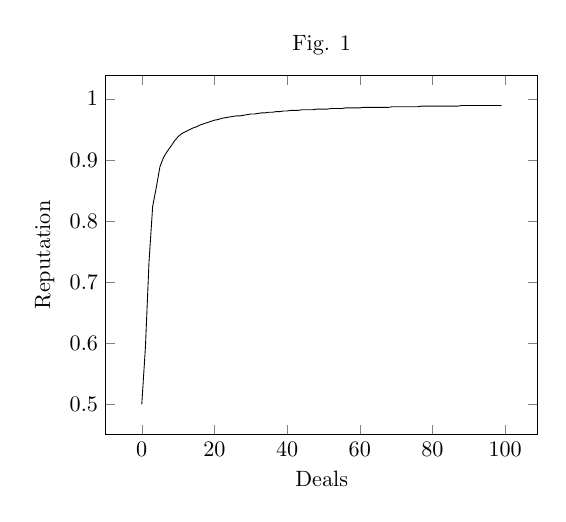
\begin{tikzpicture}[scale=0.8]
  \begin{axis}[
    title= Fig. 1,
    % xlabel=$x$ coordinate,
    xlabel=Deals,
    ylabel=Reputation,]
    \addplot [black,mark=.] coordinates {(0.000, 0.500) (1.000, 0.593) (2.000, 0.734) (3.000, 0.824) (4.000, 0.855) (5.000, 0.889) (6.000, 0.904) (7.000, 0.914) (8.000, 0.922) (9.000, 0.931) (10.000, 0.938) (11.000, 0.943) (12.000, 0.946) (13.000, 0.949) (14.000, 0.952) (15.000, 0.954) (16.000, 0.957) (17.000, 0.959) (18.000, 0.961) (19.000, 0.963) (20.000, 0.965) (21.000, 0.966) (22.000, 0.968) (23.000, 0.969) (24.000, 0.970) (25.000, 0.971) (26.000, 0.972) (27.000, 0.972) (28.000, 0.973) (29.000, 0.974) (30.000, 0.975) (31.000, 0.975) (32.000, 0.976) (33.000, 0.977) (34.000, 0.977) (35.000, 0.978) (36.000, 0.978) (37.000, 0.979) (38.000, 0.979) (39.000, 0.980) (40.000, 0.980) (41.000, 0.981) (42.000, 0.981) (43.000, 0.981) (44.000, 0.982) (45.000, 0.982) (46.000, 0.982) (47.000, 0.982) (48.000, 0.983) (49.000, 0.983) (50.000, 0.983) (51.000, 0.983) (52.000, 0.984) (53.000, 0.984) (54.000, 0.984) (55.000, 0.984) (56.000, 0.985) (57.000, 0.985) (58.000, 0.985) (59.000, 0.985) (60.000, 0.985) (61.000, 0.986) (62.000, 0.986) (63.000, 0.986) (64.000, 0.986) (65.000, 0.986) (66.000, 0.986) (67.000, 0.986) (68.000, 0.986) (69.000, 0.987) (70.000, 0.987) (71.000, 0.987) (72.000, 0.987) (73.000, 0.987) (74.000, 0.987) (75.000, 0.987) (76.000, 0.987) (77.000, 0.988) (78.000, 0.988) (79.000, 0.988) (80.000, 0.988) (81.000, 0.988) (82.000, 0.988) (83.000, 0.988) (84.000, 0.988) (85.000, 0.988) (86.000, 0.988) (87.000, 0.988) (88.000, 0.989) (89.000, 0.989) (90.000, 0.989) (91.000, 0.989) (92.000, 0.989) (93.000, 0.989) (94.000, 0.989) (95.000, 0.989) (96.000, 0.989) (97.000, 0.989) (98.000, 0.989) (99.000, 0.989)};
  \end{axis}
\end{tikzpicture}
\hspace{1cm}
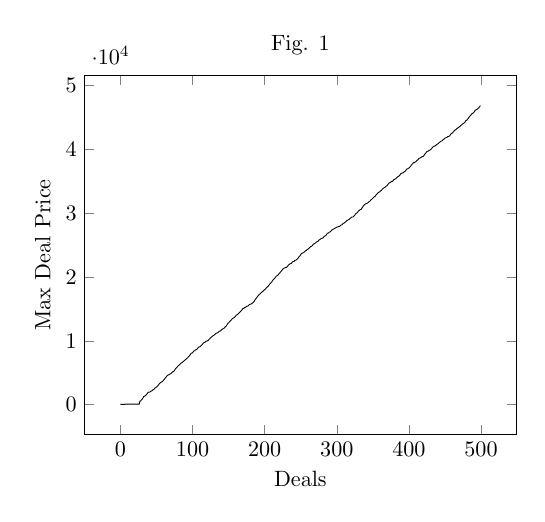
\begin{tikzpicture}[scale=0.8]
  \begin{axis}[
    title= Fig. 1,
    % xlabel=$x$ coordinate,
    xlabel=Deals,
    ylabel=Max Deal Price,]
    \addplot [black,mark=.] coordinates {(0.000, 50.000) (1.000, 50.921) (2.000, 50.921) (3.000, 50.921) (4.000, 50.921) (5.000, 50.921) (6.000, 50.921) (7.000, 82.331) (8.000, 82.331) (9.000, 85.452) (10.000, 89.604) (11.000, 89.604) (12.000, 89.604) (13.000, 92.094) (14.000, 92.094) (15.000, 92.094) (16.000, 92.094) (17.000, 92.387) (18.000, 92.387) (19.000, 93.163) (20.000, 93.163) (21.000, 93.163) (22.000, 93.809) (23.000, 93.809) (24.000, 93.809) (25.000, 93.809) (26.000, 94.148) (27.000, 567.271) (28.000, 594.923) (29.000, 751.828) (30.000, 868.901) (31.000, 1018.037) (32.000, 1252.683) (33.000, 1311.253) (34.000, 1376.995) (35.000, 1479.340) (36.000, 1564.634) (37.000, 1734.843) (38.000, 1884.807) (39.000, 1955.742) (40.000, 1962.634) (41.000, 2001.555) (42.000, 2102.621) (43.000, 2130.543) (44.000, 2213.257) (45.000, 2342.310) (46.000, 2371.735) (47.000, 2495.167) (48.000, 2634.565) (49.000, 2697.398) (50.000, 2777.580) (51.000, 2888.197) (52.000, 2982.159) (53.000, 3132.516) (54.000, 3303.934) (55.000, 3398.891) (56.000, 3490.918) (57.000, 3566.243) (58.000, 3595.443) (59.000, 3738.769) (60.000, 3891.556) (61.000, 3995.632) (62.000, 4181.373) (63.000, 4274.354) (64.000, 4445.084) (65.000, 4596.563) (66.000, 4654.314) (67.000, 4683.564) (68.000, 4754.961) (69.000, 4831.600) (70.000, 4881.949) (71.000, 4991.724) (72.000, 5133.725) (73.000, 5137.648) (74.000, 5252.465) (75.000, 5389.109) (76.000, 5573.392) (77.000, 5725.986) (78.000, 5829.074) (79.000, 5960.440) (80.000, 6086.563) (81.000, 6185.304) (82.000, 6272.202) (83.000, 6383.063) (84.000, 6515.798) (85.000, 6576.315) (86.000, 6642.985) (87.000, 6749.572) (88.000, 6858.550) (89.000, 6958.310) (90.000, 7057.416) (91.000, 7120.796) (92.000, 7249.946) (93.000, 7342.745) (94.000, 7470.393) (95.000, 7572.635) (96.000, 7735.256) (97.000, 7853.908) (98.000, 8068.636) (99.000, 8104.137) (100.000, 8122.206) (101.000, 8313.333) (102.000, 8431.730) (103.000, 8472.115) (104.000, 8597.731) (105.000, 8600.850) (106.000, 8689.991) (107.000, 8822.244) (108.000, 8971.471) (109.000, 9059.329) (110.000, 9076.932) (111.000, 9144.711) (112.000, 9296.032) (113.000, 9392.970) (114.000, 9512.232) (115.000, 9670.604) (116.000, 9738.462) (117.000, 9749.746) (118.000, 9875.477) (119.000, 9969.006) (120.000, 9971.813) (121.000, 10059.673) (122.000, 10089.950) (123.000, 10267.423) (124.000, 10343.065) (125.000, 10478.507) (126.000, 10583.331) (127.000, 10669.887) (128.000, 10798.045) (129.000, 10835.559) (130.000, 10919.757) (131.000, 11007.021) (132.000, 11139.318) (133.000, 11206.475) (134.000, 11241.267) (135.000, 11298.147) (136.000, 11402.990) (137.000, 11522.547) (138.000, 11546.702) (139.000, 11575.638) (140.000, 11747.102) (141.000, 11801.406) (142.000, 11908.859) (143.000, 11911.309) (144.000, 12042.957) (145.000, 12165.948) (146.000, 12245.620) (147.000, 12387.549) (148.000, 12573.185) (149.000, 12761.091) (150.000, 12824.315) (151.000, 12988.461) (152.000, 13081.626) (153.000, 13188.760) (154.000, 13323.848) (155.000, 13462.263) (156.000, 13550.539) (157.000, 13600.833) (158.000, 13694.786) (159.000, 13786.867) (160.000, 13939.566) (161.000, 14061.209) (162.000, 14121.109) (163.000, 14199.105) (164.000, 14310.709) (165.000, 14428.218) (166.000, 14567.570) (167.000, 14659.802) (168.000, 14798.219) (169.000, 14961.486) (170.000, 15091.455) (171.000, 15093.657) (172.000, 15200.430) (173.000, 15241.008) (174.000, 15320.790) (175.000, 15422.029) (176.000, 15435.346) (177.000, 15469.383) (178.000, 15629.777) (179.000, 15693.332) (180.000, 15743.754) (181.000, 15774.996) (182.000, 15840.473) (183.000, 15936.879) (184.000, 15991.696) (185.000, 16144.358) (186.000, 16329.804) (187.000, 16517.042) (188.000, 16654.932) (189.000, 16787.635) (190.000, 16945.353) (191.000, 17094.258) (192.000, 17208.912) (193.000, 17316.897) (194.000, 17418.308) (195.000, 17543.345) (196.000, 17635.404) (197.000, 17749.233) (198.000, 17791.786) (199.000, 17957.681) (200.000, 18040.012) (201.000, 18106.618) (202.000, 18269.294) (203.000, 18403.074) (204.000, 18492.847) (205.000, 18569.005) (206.000, 18749.377) (207.000, 18900.043) (208.000, 19027.066) (209.000, 19162.234) (210.000, 19260.243) (211.000, 19465.578) (212.000, 19582.545) (213.000, 19704.216) (214.000, 19820.398) (215.000, 19986.440) (216.000, 20112.796) (217.000, 20217.333) (218.000, 20297.000) (219.000, 20376.780) (220.000, 20572.383) (221.000, 20661.884) (222.000, 20822.866) (223.000, 20936.101) (224.000, 21076.883) (225.000, 21235.878) (226.000, 21317.424) (227.000, 21413.287) (228.000, 21442.664) (229.000, 21514.040) (230.000, 21530.116) (231.000, 21620.468) (232.000, 21735.507) (233.000, 21913.261) (234.000, 21953.885) (235.000, 22081.174) (236.000, 22110.922) (237.000, 22157.854) (238.000, 22288.422) (239.000, 22423.349) (240.000, 22446.018) (241.000, 22494.533) (242.000, 22632.644) (243.000, 22637.800) (244.000, 22704.688) (245.000, 22828.346) (246.000, 22922.852) (247.000, 23102.989) (248.000, 23222.420) (249.000, 23341.697) (250.000, 23532.814) (251.000, 23691.071) (252.000, 23739.148) (253.000, 23810.190) (254.000, 23836.596) (255.000, 23961.680) (256.000, 24063.589) (257.000, 24146.173) (258.000, 24208.339) (259.000, 24315.431) (260.000, 24382.565) (261.000, 24474.643) (262.000, 24598.677) (263.000, 24712.563) (264.000, 24786.929) (265.000, 24847.370) (266.000, 24921.568) (267.000, 25091.497) (268.000, 25206.336) (269.000, 25235.734) (270.000, 25321.229) (271.000, 25413.675) (272.000, 25543.977) (273.000, 25545.484) (274.000, 25630.456) (275.000, 25801.810) (276.000, 25843.161) (277.000, 25928.238) (278.000, 26010.799) (279.000, 26056.033) (280.000, 26102.918) (281.000, 26149.680) (282.000, 26322.147) (283.000, 26395.672) (284.000, 26471.100) (285.000, 26554.028) (286.000, 26695.605) (287.000, 26860.716) (288.000, 26892.106) (289.000, 26951.835) (290.000, 27061.953) (291.000, 27101.985) (292.000, 27238.765) (293.000, 27372.131) (294.000, 27414.768) (295.000, 27512.249) (296.000, 27551.194) (297.000, 27643.623) (298.000, 27686.059) (299.000, 27770.209) (300.000, 27825.614) (301.000, 27849.206) (302.000, 27896.389) (303.000, 27960.050) (304.000, 27961.392) (305.000, 28073.518) (306.000, 28161.235) (307.000, 28177.936) (308.000, 28305.734) (309.000, 28437.565) (310.000, 28454.878) (311.000, 28544.818) (312.000, 28639.881) (313.000, 28757.851) (314.000, 28849.099) (315.000, 28915.347) (316.000, 28992.359) (317.000, 29035.059) (318.000, 29148.119) (319.000, 29230.797) (320.000, 29337.864) (321.000, 29412.025) (322.000, 29413.272) (323.000, 29466.469) (324.000, 29576.495) (325.000, 29719.728) (326.000, 29892.654) (327.000, 30004.945) (328.000, 30048.319) (329.000, 30193.715) (330.000, 30345.948) (331.000, 30440.478) (332.000, 30538.060) (333.000, 30600.649) (334.000, 30640.002) (335.000, 30879.427) (336.000, 31010.145) (337.000, 31176.968) (338.000, 31299.088) (339.000, 31398.971) (340.000, 31480.488) (341.000, 31532.963) (342.000, 31572.662) (343.000, 31643.306) (344.000, 31721.167) (345.000, 31846.390) (346.000, 31908.213) (347.000, 32064.951) (348.000, 32157.178) (349.000, 32273.651) (350.000, 32384.851) (351.000, 32489.801) (352.000, 32610.503) (353.000, 32617.522) (354.000, 32818.973) (355.000, 32940.284) (356.000, 33051.281) (357.000, 33190.901) (358.000, 33287.240) (359.000, 33329.973) (360.000, 33437.320) (361.000, 33554.531) (362.000, 33594.255) (363.000, 33780.198) (364.000, 33880.077) (365.000, 33947.867) (366.000, 34035.158) (367.000, 34092.091) (368.000, 34203.030) (369.000, 34284.968) (370.000, 34370.042) (371.000, 34556.107) (372.000, 34658.845) (373.000, 34771.141) (374.000, 34796.570) (375.000, 34904.666) (376.000, 35004.817) (377.000, 35006.327) (378.000, 35086.062) (379.000, 35268.991) (380.000, 35296.807) (381.000, 35386.756) (382.000, 35414.936) (383.000, 35570.172) (384.000, 35668.745) (385.000, 35777.819) (386.000, 35806.296) (387.000, 35930.889) (388.000, 36068.779) (389.000, 36235.783) (390.000, 36260.489) (391.000, 36316.925) (392.000, 36340.871) (393.000, 36451.650) (394.000, 36545.054) (395.000, 36603.188) (396.000, 36783.430) (397.000, 36946.607) (398.000, 36947.462) (399.000, 37066.149) (400.000, 37080.256) (401.000, 37208.032) (402.000, 37332.780) (403.000, 37481.364) (404.000, 37602.491) (405.000, 37787.027) (406.000, 37876.408) (407.000, 37982.445) (408.000, 37983.252) (409.000, 38045.100) (410.000, 38137.930) (411.000, 38275.879) (412.000, 38353.158) (413.000, 38441.603) (414.000, 38630.515) (415.000, 38631.290) (416.000, 38713.956) (417.000, 38770.865) (418.000, 38870.945) (419.000, 38888.839) (420.000, 38926.758) (421.000, 39093.989) (422.000, 39261.662) (423.000, 39382.569) (424.000, 39530.754) (425.000, 39692.774) (426.000, 39732.055) (427.000, 39749.306) (428.000, 39845.503) (429.000, 39908.989) (430.000, 39953.178) (431.000, 40077.533) (432.000, 40217.078) (433.000, 40330.300) (434.000, 40505.778) (435.000, 40517.875) (436.000, 40540.392) (437.000, 40651.506) (438.000, 40695.874) (439.000, 40814.307) (440.000, 40873.464) (441.000, 40958.784) (442.000, 41092.227) (443.000, 41148.239) (444.000, 41252.533) (445.000, 41321.478) (446.000, 41359.671) (447.000, 41475.654) (448.000, 41597.961) (449.000, 41645.271) (450.000, 41790.194) (451.000, 41821.065) (452.000, 41876.802) (453.000, 41920.892) (454.000, 42046.957) (455.000, 42047.544) (456.000, 42095.091) (457.000, 42205.696) (458.000, 42402.765) (459.000, 42483.214) (460.000, 42584.209) (461.000, 42703.520) (462.000, 42785.423) (463.000, 42961.218) (464.000, 43058.354) (465.000, 43086.629) (466.000, 43240.472) (467.000, 43318.542) (468.000, 43390.124) (469.000, 43484.651) (470.000, 43546.548) (471.000, 43633.846) (472.000, 43788.216) (473.000, 43841.460) (474.000, 43946.218) (475.000, 44042.088) (476.000, 44136.533) (477.000, 44177.548) (478.000, 44319.005) (479.000, 44522.094) (480.000, 44576.594) (481.000, 44690.601) (482.000, 44819.413) (483.000, 44999.222) (484.000, 45143.099) (485.000, 45279.285) (486.000, 45377.850) (487.000, 45585.392) (488.000, 45622.800) (489.000, 45719.047) (490.000, 45802.415) (491.000, 45970.275) (492.000, 46157.742) (493.000, 46199.685) (494.000, 46277.559) (495.000, 46333.611) (496.000, 46446.859) (497.000, 46530.543) (498.000, 46675.221) (499.000, 46902.682)};
  \end{axis}
\end{tikzpicture}
\end{center}

Figure 1 shows a simplified scenario of how a user's reputation grows if he makes evenly priced deals. Figure 2 shows how a user's maximum deal price grows as he makes successful deals.

\subsection{Single buyer: fraud and recovery scenarios} \label{appendix:fraudAndRecovery}

Lorem ipsum.


\newpage

\begin{thebibliography}{1}
 
\bibitem{josang2002beta} 
Josang, Audun and Ismail, Roslan. 
\textit{The beta reputation system}.
Proceedings of the 15th bled electronic commerce conference, Vol. 5, p.2502--2511, 2002.

\bibitem{ciccarelli2011collusion}
Ciccarelli, Gianluca and Cigno, Renato Lo.
\textit{Collusion in peer-to-peer systems}.
Computer Networks, vol. 55, ?15, p.3517--3532, 2011.

\bibitem{maranzato2010fraud}
Maranzato, Rafael and Pereira, Adriano and do Lago, Alair Pereira and Neubert, Marden.
\textit{Fraud detection in reputation systems in e-markets using logistic regression.}
Proceedings of the 2010 ACM Symposium on Applied Computing, p.1454--1455, 2010.

\end{thebibliography}

\end{document}